%!TEX program = xelatex
\documentclass{beamer}

\usepackage[english]{babel}

\usepackage[export]{adjustbox}
\usepackage{graphicx,hyperref,url, materialbeamer}
\usepackage{braket}
%\usepackage{euler}
\usepackage{listings}


\graphicspath{ {./images/} }
%\setbeamercovered{transparent}



\usefonttheme{professionalfonts} % using non standard fonts for beamer
%\usefonttheme{serif}

% The title of the presentation:
%  - first a short version which is visible at the bottom of each slide;
%  - second the full title shown on the title slide;
\title[LOGwear Demo Facility]{Demo Facility}

% Optional: a subtitle to be dispalyed on the title slide
\subtitle{Wearables in Logistics}

% The author(s) of the presentation:
%  - again first a short version to be displayed at the bottom;
%  - next the full list of authors, which may include contact information;
\author[L. Rolle]{Lukas Rolle - 2310309} 
  
%\titlegraphic{\includegraphics[width=\textwidth]{atac-logo}}

% The institute:
%  - to start the name of the university as displayed on the top of each slide
%    this can be adjusted such that you can also create a Dutch version
%  - next the institute information as displayed on the title slide
\institute[FHTenL]{
Sofware Engineering\\
  Bachelor Thesis - Midterm presentation \\
  Fontys Hogeschool Techniek en Logistiek}

% Add a date and possibly the name of the event to the slides
%  - again first a short version to be shown at the bottom of each slide
%  - second the full date and event name for the title slide
\date[\today]{
 \today}



\providecommand{\di}{\mathop{}\!\mathrm{d}}
\providecommand*{\der}[3][]{\frac{d\if?#1?\else^{#1}\fi#2}{d #3\if?#1?\else^{#1}\fi}} 
 \providecommand*{\pder}[3][]{% 
    \frac{\partial\if?#1?\else^{#1}\fi#2}{\partial #3\if?#1?\else^{#1}\fi}% 
  }
\begin{document}

\begin{frame}
  \titlepage
\end{frame}

\begin{frame}
  \frametitle{Table of Contents}

  \tableofcontents
\end{frame}

\setlength{\parskip}{\baselineskip} 

\chapter{Introduction}\pagenumbering{arabic}
This document is the project plan for the creation of a demo facility for the LOGwear project.

\section{LOGwear}

\noindent LOGwear is a research project that aims to bring wearables to the area of logistics, especially to \gls{sme}. It is a German-Dutch research project were multiple parties are cooperating to create results. Involved in this are two Universities of applied sciences, \gls{fhtenl} in Venlo as the lead partner, Netherlands and \gls{hsnr} in Krefeld, Germany.

Further on there are also multiple partner companies involved in the project, namely KLG Europe bv, Helmut Beyers GmbH and imat-uve GmbH. These partner companies are there to give the knowledge about logistics processes, as well as to verify and test the results.

The project is backed within the scope of the INTERREG Deutschland-Nederland initiative. It is backed by the \gls{eu}, \gls{mweimh} and the Provincie Limburg as well.



\section{Demo Facility}
The demo facility that should be created for this project will be a physical environment in which a logistics process can be modelled. This process should then be improved by using a wearable. This will be used as a demonstration area for \gls{sme} to see hands-on, if a wearable could be used to improve their own processes. The demo facility will be a proof of concept and not a fully implemented solution that could be directly used at a logistics company and instantly work.

\section{Schedule}
The initial schedule for the project can be seen in table \ref{tab:schedule}. It is to be mentioned, that the schedule is subject to change as the project goes on. The project will be executed in a scrum-like way that is adapted to the group, given the group size of two developers.
\begin{table}[htbp]
\centering
\large
\resizebox{1\textwidth}{!} {
\begin{tabular}{|c"cc:cccc:cc:ccccccccc:ccc:c|} \hline
\textbf{Sprints} & \multicolumn{2}{>{\centering\arraybackslash} m{.15\textwidth}|}{\textbf{Logistics Processes \& Wearables}} & \multicolumn{4}{>{\centering\arraybackslash} m{.35\textwidth}|}{\textbf{Reference Architecture}} & \multicolumn{2}{>{\centering\arraybackslash} m{.25\textwidth}|}{\textbf{Research Demo Facility}} & \multicolumn{9}{c|}{\textbf{Demo Facility Design and Implementation}}                   & \multicolumn{3}{>{\centering\arraybackslash} m{.25\textwidth}|}{\textbf{Creation Demo Facility}} & \multicolumn{1}{>{\centering\arraybackslash} m{.08\textwidth}|}{\textbf{Buf-fer}} \\ \thickhline
Date                 & 06.02              & 13.02              & 20.02                & 27.02                & 06.03         & 13.03        & 20.03        & 27.03 & 03.04 & 10.04 & 17.04 & 24.04 & 01.05 & 08.05 & 15.05 & 22.05 & 29.05 & 05.06         & 12.06        & 19.06        & 26.06                             \\
Week                       & 6                  & 7                  & 8                    & 9                    & 10            & 11           & 12           & 13    & 14    & 15    & 16    & 17    & 18    & 19    & 20    & 21    & 22    & 23            & 24           & 25           & 26 \\\hline       	              
\end{tabular}
}
\caption{Schedule}
\label{tab:schedule}
\end{table}

The schedule is divided in work packages that are to be executed, it is to be noted, that each work package could be split into multiple sprints in the future. In the following subsections the work packages will be explained.

\subsection{Logistics Processes \& Wearables}
This work package includes research about the gives processes and wearables in general, as well as already choosing potential wearables that could be used to improve the process. The end result for this should be a decision on process and wearable. But the result for this could potentially take longer than this task is scheduled. The wearables should be ranked after getting hands-on experience on them, therefore some of them have to be ordered first.

\subsection{Reference Architecture}
A reference architecture should be created for a sample wearable application. What this work package contains is, the creation of diagrams which show the communication from a wearable to the \gls{wms} or something similar. What should not be created is a full reference architecture for a process that is implemented with a concrete wearable. 

It is about creating the always needed layers when using a wearable in a way that supports most wearable solutions.

\subsection{Research Demo Facility}
This task includes researching what physical objects and what systems would be needed to create a demo facility that could showcase a single process with a single wearable. This also includes the gathering of knowledge of where the demo facility should be created and where to get the needed objects.

\subsection{Demo Facility Design and Implementation}
The work package includes the creation of the software design and implementation for the wearable and all aspects that are needed to fully showcase a process.

\subsection{Creation Demo Facility}
This task includes the physical creation of the demo facility. This means setting up shelves with packages to scan and put on a hand pallet truck. Setting up barcodes on the packages to scan. Setting up an environment that can showcase what is happening better to an audience.


\section{Overview}
In this section the following chapters will be shortly explained. 

The first chapter following this, chapter \ref{cha:scope} is about the scope of the assignment. The risk management done in the project will be explained in chapter \ref{cha:riskManagement}. The last chapter will be about the existing stakeholders in the chapter \ref{cha:stakeholders}.
%\section{Approach}
\begin{frame}\frametitle{Approach}
	\begin{itemize}
		\item Scrum-like
		\begin{itemize}
			\item Adapted to group size
			\item No stand-up meetings
		\end{itemize}
		\item Up to this point as single developer
		\begin{itemize}
			\item In the future a development team of two developers
		\end{itemize}
	\end{itemize}
\end{frame}
\begin{frame}\frametitle{Schedule}
\begin{figure}
	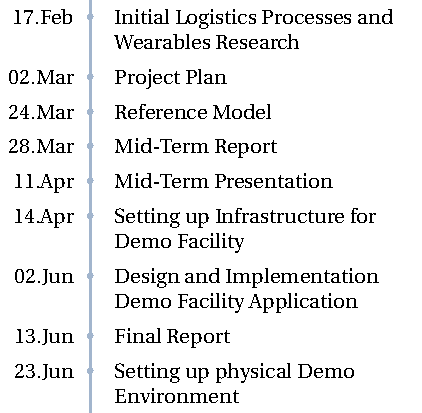
\includegraphics[scale=0.9]{images/TimeLine}
\end{figure}
\end{frame}
\section{Research}
\begin{frame}\frametitle{Research}
	\begin{itemize}
		\item 1
	\end{itemize}
\end{frame}
\section{Reference Model}
\begin{frame}\frametitle{Reference Model}
	\begin{itemize}
		\item Single Model
	\end{itemize}
	\begin{itemize}
		\item Abstract
		\item Flexibility
		\begin{itemize}
			\item Allow changes if needed
		\end{itemize}
	\end{itemize}
\end{frame}
\begin{frame}\frametitle{Reference Model}
	\begin{figure}
		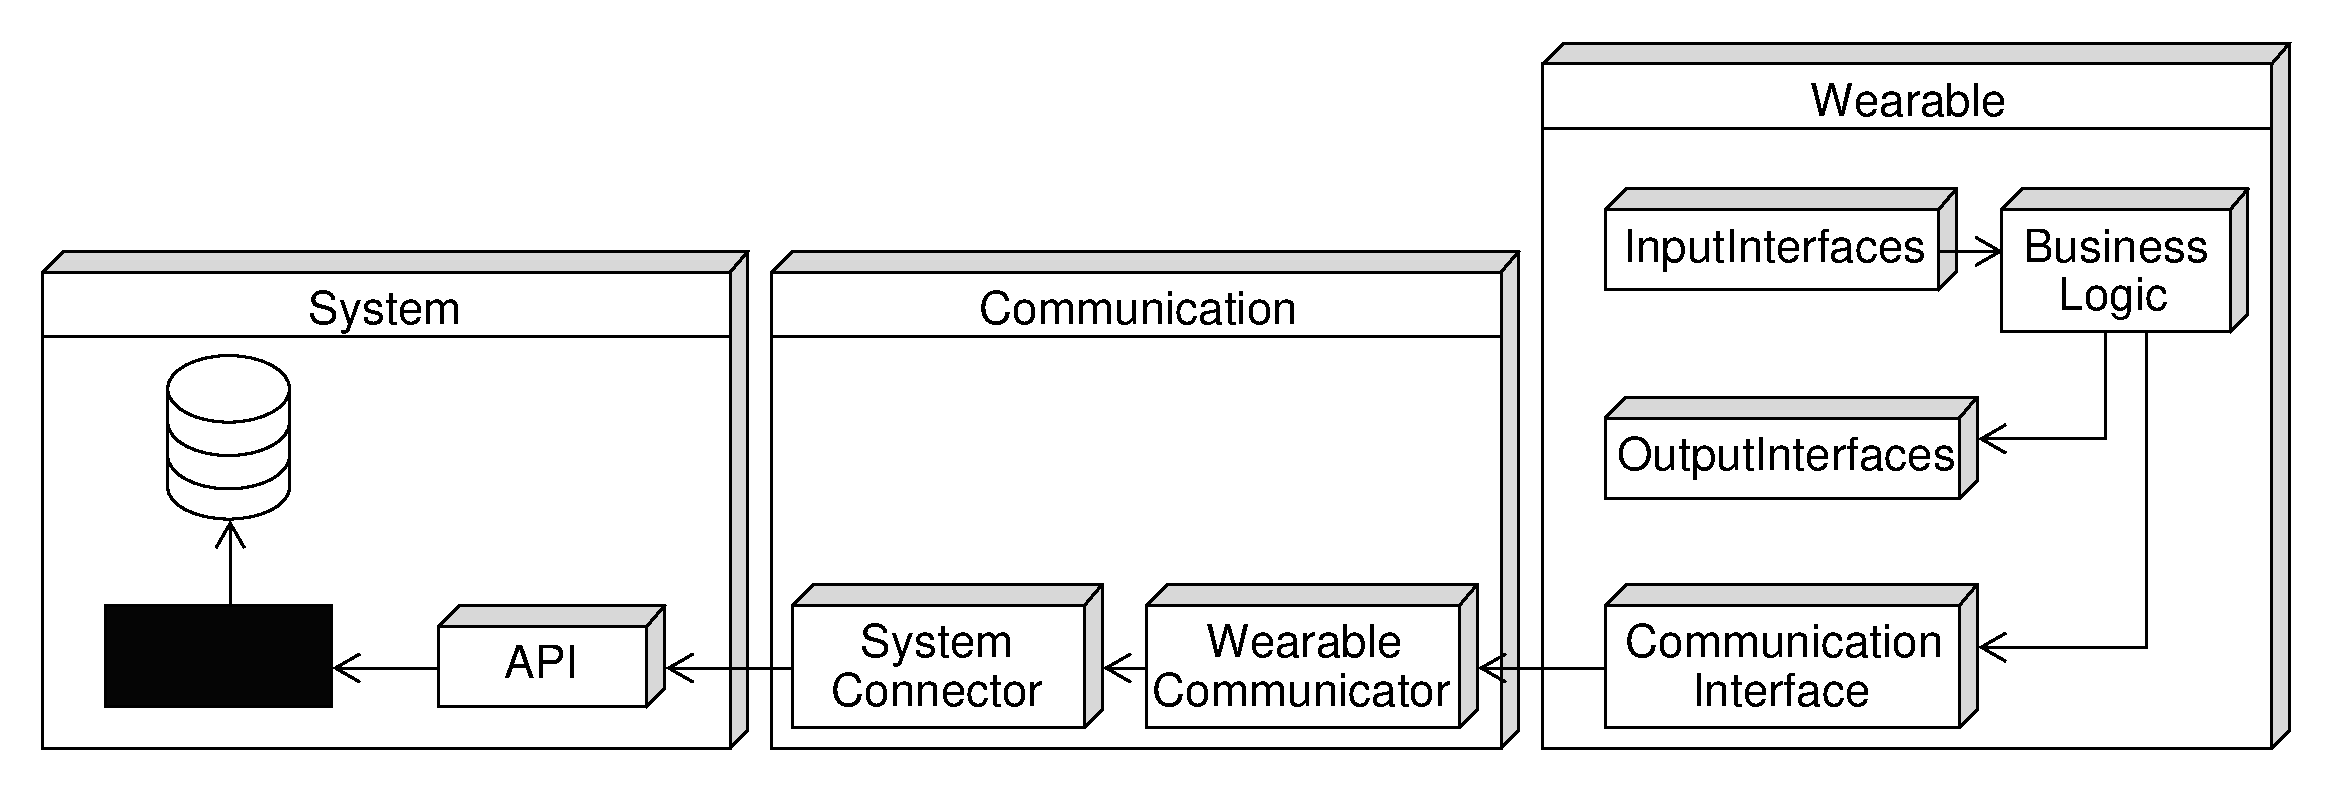
\includegraphics[width=\textwidth]{images/ReferenceModel}
	\end{figure}
\end{frame}
\begin{frame}\frametitle{Reference Model Examples}
	\begin{figure}
		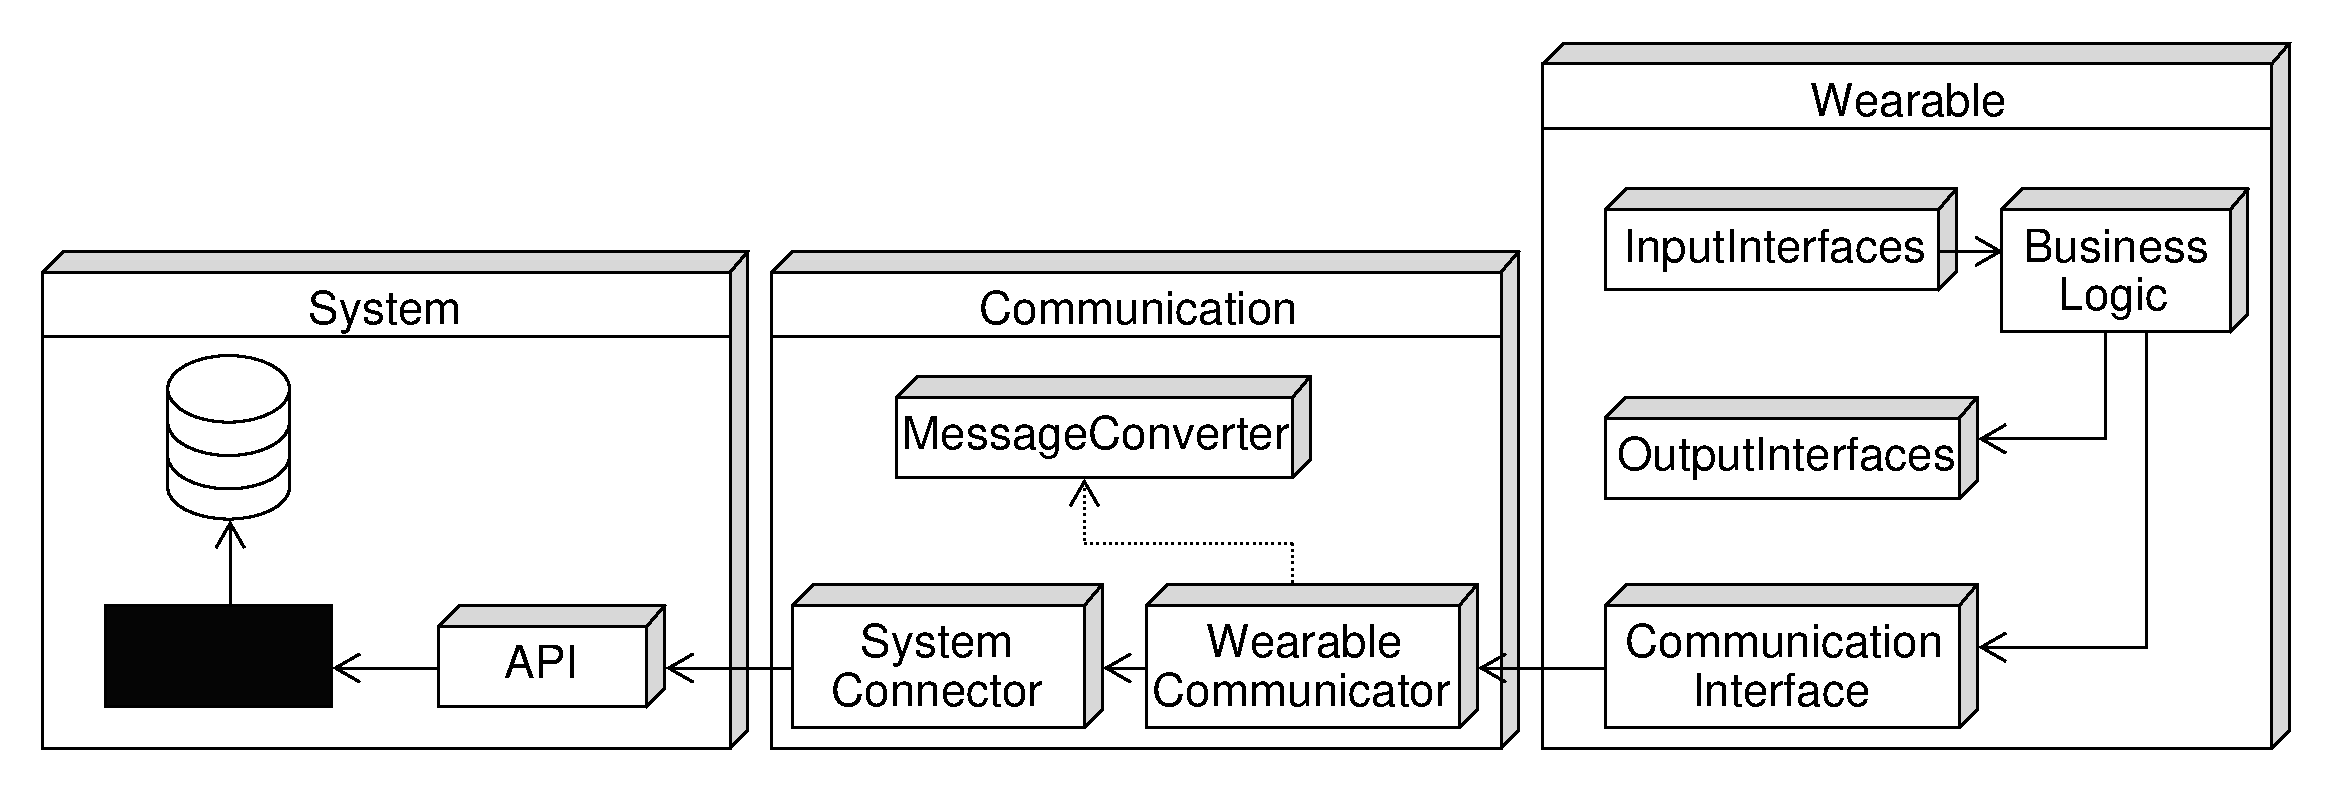
\includegraphics[width=\textwidth]{images/ReferenceModel_Converter}
	\end{figure}
\end{frame}
\begin{frame}\frametitle{Reference Model Examples}
	\begin{figure}
		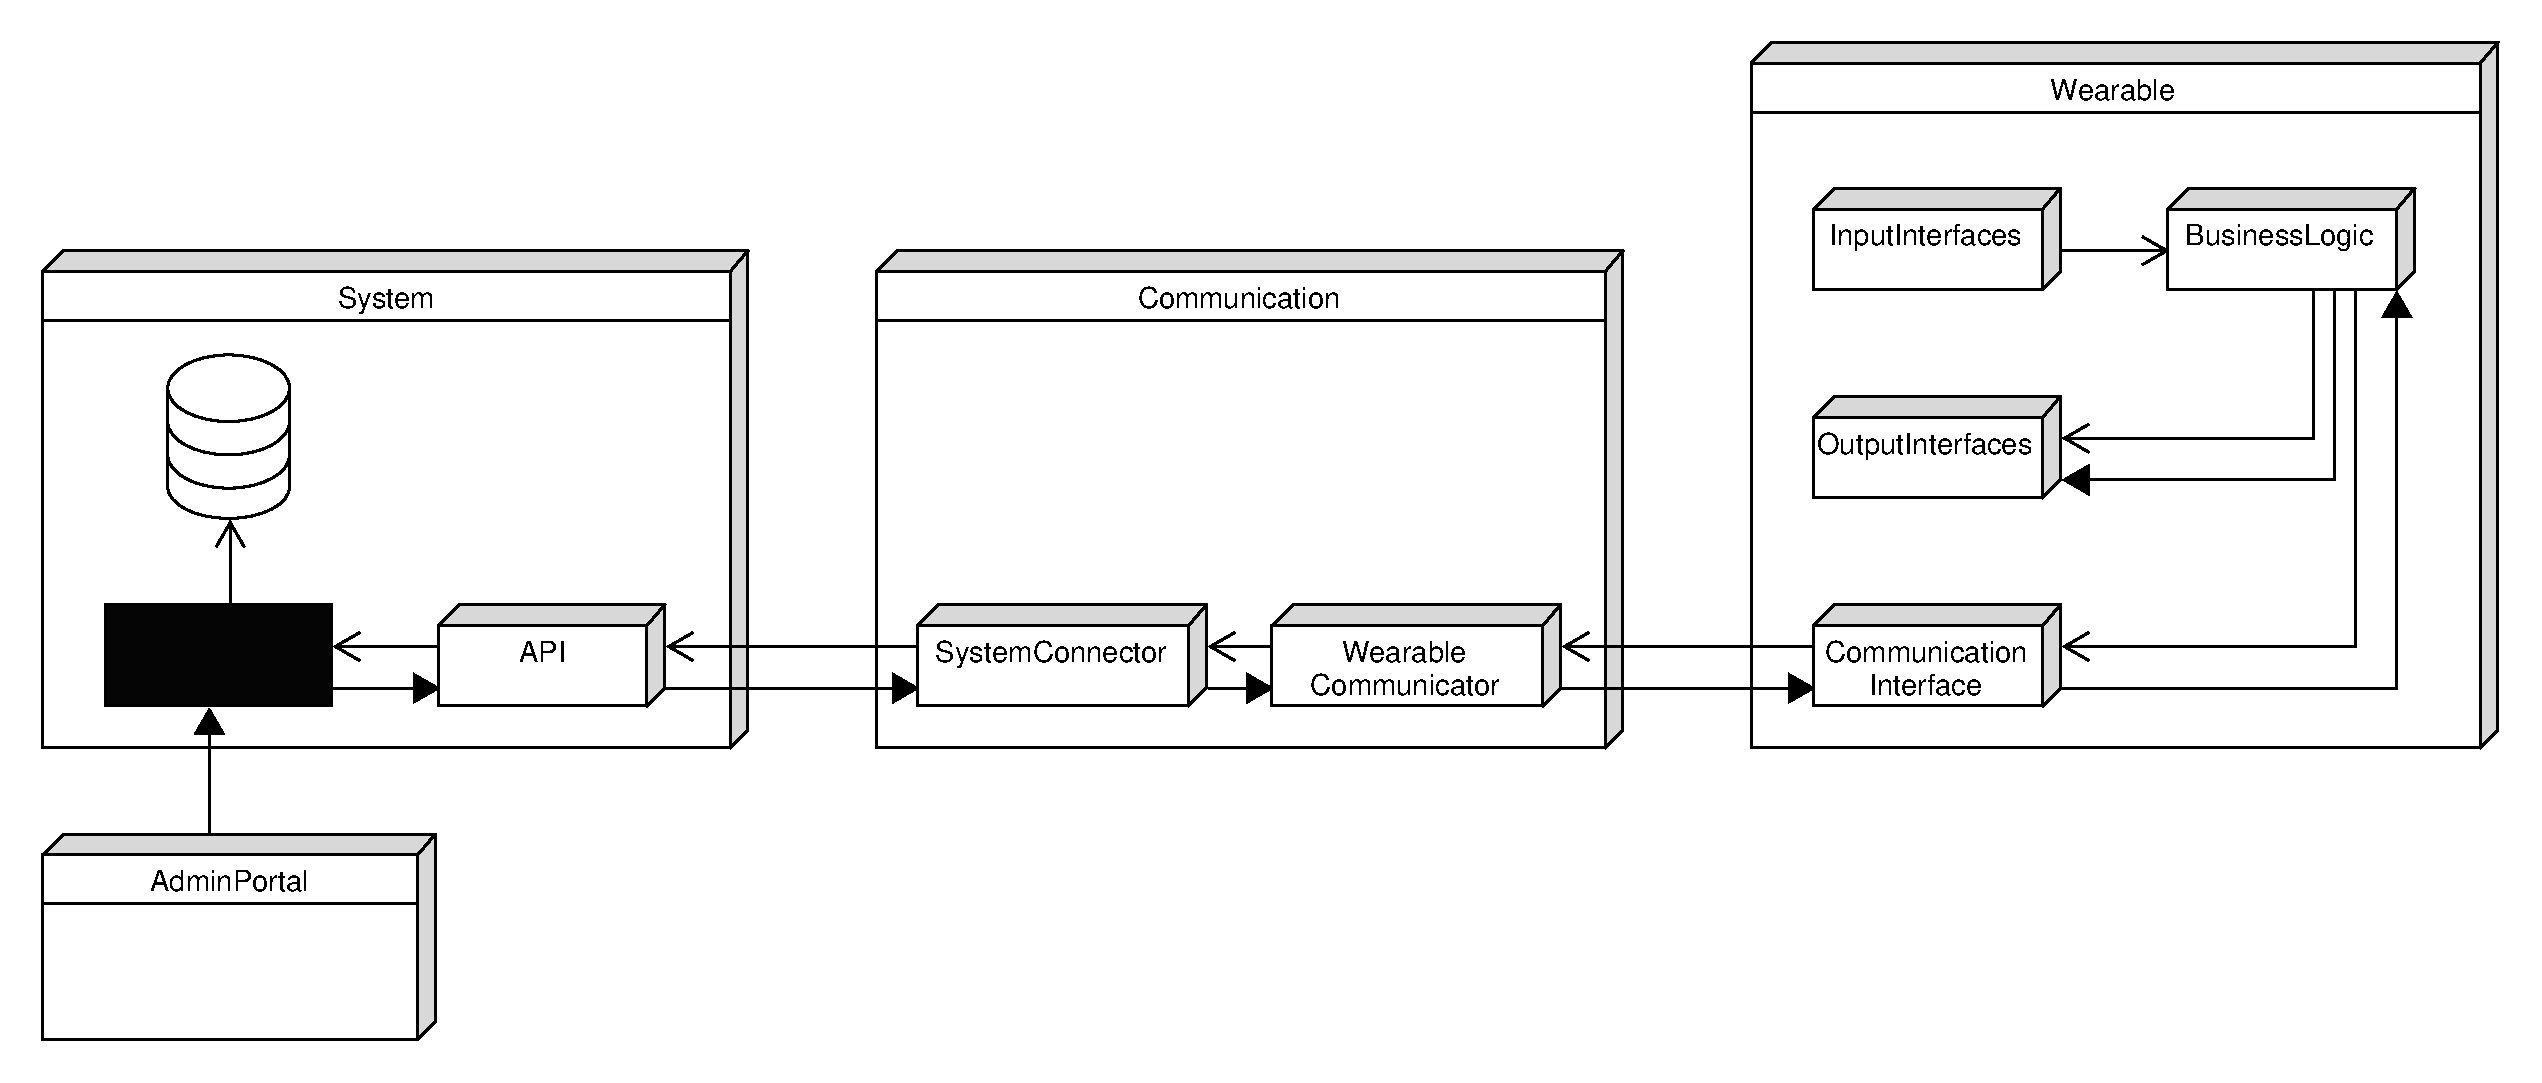
\includegraphics[width=\textwidth]{images/PackageModel_ReferenceArchitecture_PushMessages}
	\end{figure}
\end{frame}

\chapter{Demo Facility}\label{cha:demoFacility}
Physical creation of the demo facility that showcases the possibilities of the chosen wearable in the process of order picking in a warehouse. As the demo facility is not yet existing the implementation cannot be discussed and explained here, this chapter will therefore focus on the planned infrastructure, the existing design and what is planned for the demo facility in the future. 

There is also a major difference between the demo facility task that will be explained in this report and the task given in the logwear website. \citep{website:logwear} The task that will be executed here will be creating a demo facility in a physical \gls{sandbox} environment and the task explained in the work package on the logwear homepage is about implementing the improved process, using a wearable, at a pilot company and observing the results.

\section{Infrastructure}
The infrastructure of the demo facility is divided into multiple areas:
\begin{description}
	\item[Mock WMS] \hfill \\
		A mock \gls{wms} that allows to store different orders and edit them to have a more realistic demo. While not all functionality has to given, the data has to be persistent and easily resettable to allow showcasing a demo case multiple times. The mock \gls{wms} is living on an azure server and is a \gls{mssql} database.
	\item[Rest API] \hfill \\
		A \gls{rest} \gls{api} that is used to connect to the mock \gls{wms} from an outside perspective, in this case from the communication layer, see subsection \ref{subsec:communication}.
	\item[Communication Layer] \hfill \\
		The communication layer will be living on a server with a connection to the \gls{db} \gls{api} and a connection to the wearable.
	\item[Wearable] \hfill \\
		The wearable will need to connect to the communication layer and process input and output.
\end{description}

The mock \gls{wms} and the \gls{rest} \gls{api} are insignificant parts of the implementation, therefore not a lot of thought was put into the decision on choosing these technologies was done out of curiosity for these technologies or being the most comfortable with them respectively.

\section{Demo Scenario}\label{sec:demoScenario}
The demo scenario explains the process that will be executed during the demo facility. Therefore describing the actions taken in detail, but ignoring how they will be executed, e.g. with or without a wearable. The original process can be seen in the appendix, figure \ref{fig:orderPickingProcessDiagram}. For the actual scenario for the demo facility an activity diagram was created, that can be seen in figure \ref{fig:activityDemoScenario}. 

\begin{figure}[htbp]
	\begin{center}
	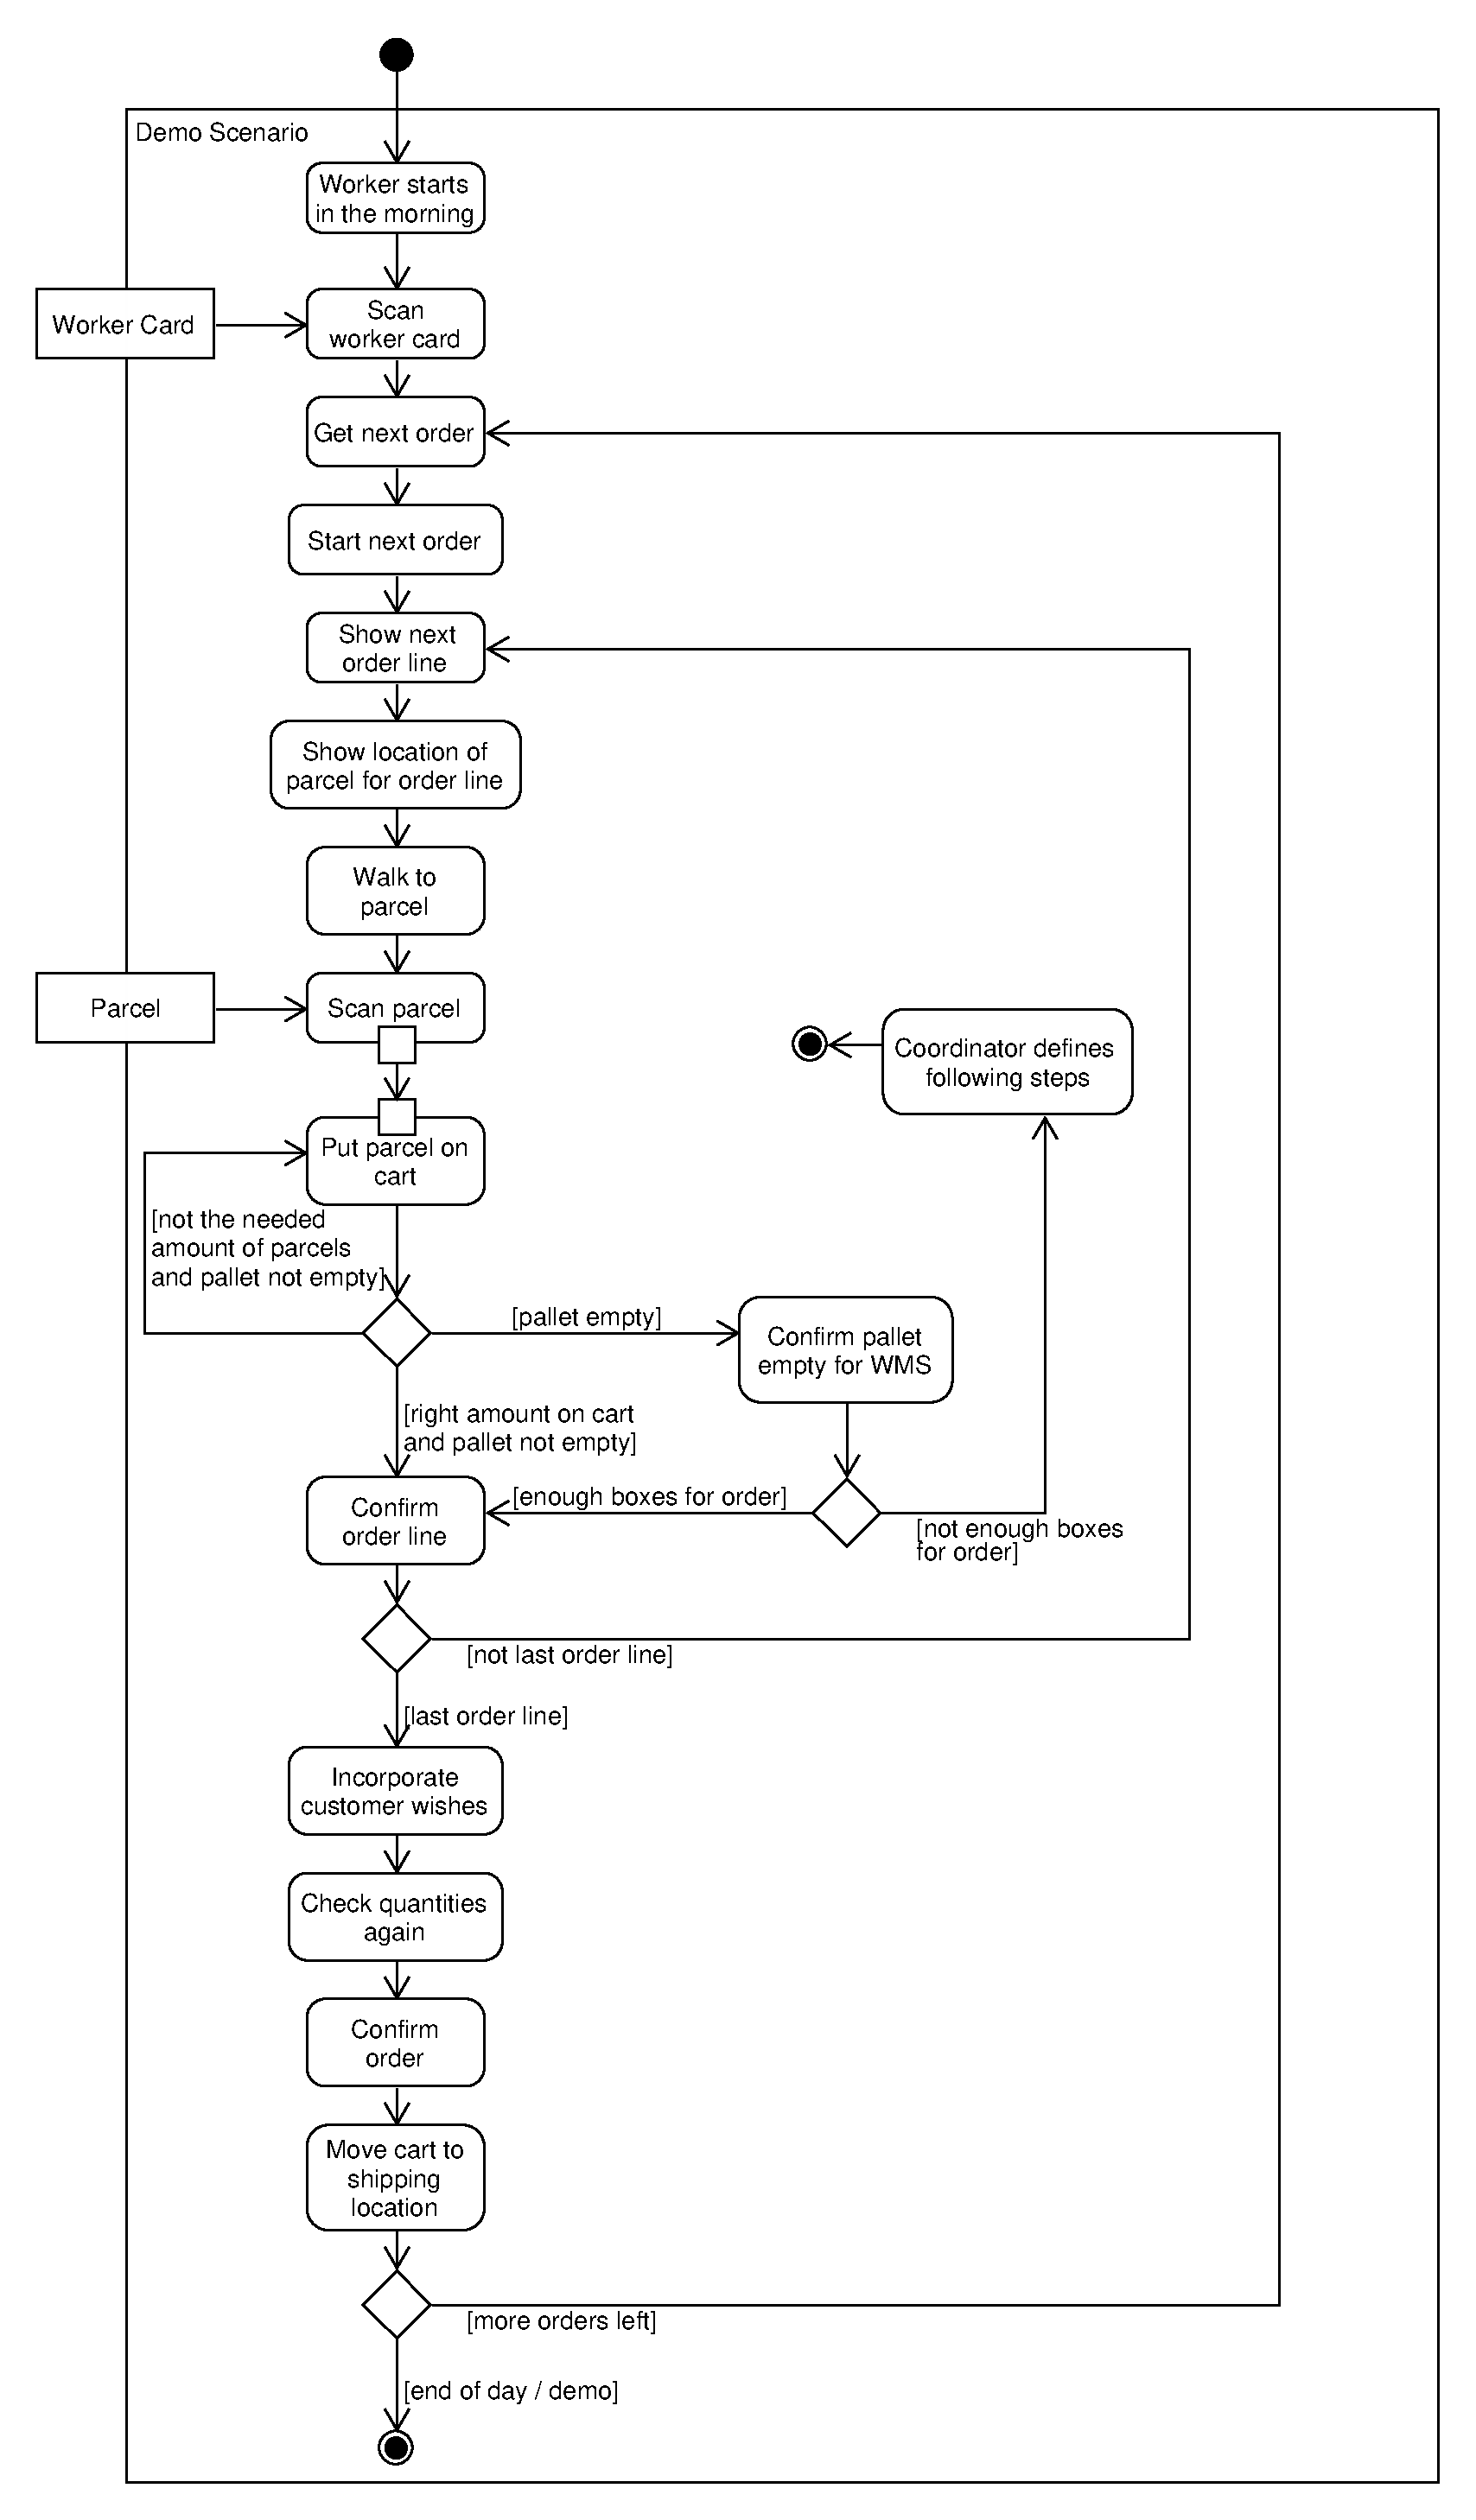
\includegraphics[height=\textheight]{images/activityDiagram_demoScenarioNoExceptions}
	\end{center}	
	\caption{Activity Diagram Demo Scenario}
	\label{fig:activityDemoScenario}
\end{figure}

\cleardoublepage

This diagram was created for multiple reasons:

\begin{description}
	\item[Readability] \hfill \\
	The scale of the original process diagram made it hard to process. One goal was to create a more compact diagram.
	\item[Purpose] \hfill \\
	The original diagram had a different purpose, it was supposed to model the process of one of the pilot companies in its entirety. The purpose of the activity diagram is to model a demo case, that does not need to show every single detail of the process in the first place.
	\item[Focus point] \hfill \\
	The demo scenario focuses on the general tasks an order picking worker is doing, but is just focussing on the main points for this. The original diagram also includes the connections to the database and also includes tasks outside of the actual order picking.
\end{description}

\textcolor{red}{add description of model}

\section{Design}
The general design for the demo facility application will be based on the reference model described in chapter \ref{cha:reference}. But in the following sections the demo facility specific design will be elaborated further.


\subsection{WMS}
The \acrlong{wms} consists of two parts, the database that is going to contain the data for the demo facility and the database connector. This also defines the interface, with which to connect to the \gls{wms}.

\subsubsection{Database}

Figure \ref{fig:LogicalModelWMS} shows the relations and fields in the database. It can be seen that the database just contains a small amount of information, due to being a demo, an actual \gls{wms} would contain a lot more data. The most important item in the model is the order, as that is the key piece, where most relations lead together. An order has a number that is connecting it to one or multiple workers that are working on them. Furthermore an order consists of multiple \texttt{OrderLine}s. An \texttt{OrderLine} is describing the different lines that would appear on an order, that specify the item and the amount for an order. For a warehouse it is also important to add the pallet where to find the item and if the current line is already acknowledged or not. A pallet has a location in the warehouse and how much of that item are still available in the warehouse. The article corresponds to a name for the article number. Finally an order is ordered by a customer, a customer might have additional wishes for their orders and an address where that customer wants things delivered to.

\begin{figure}[H]
	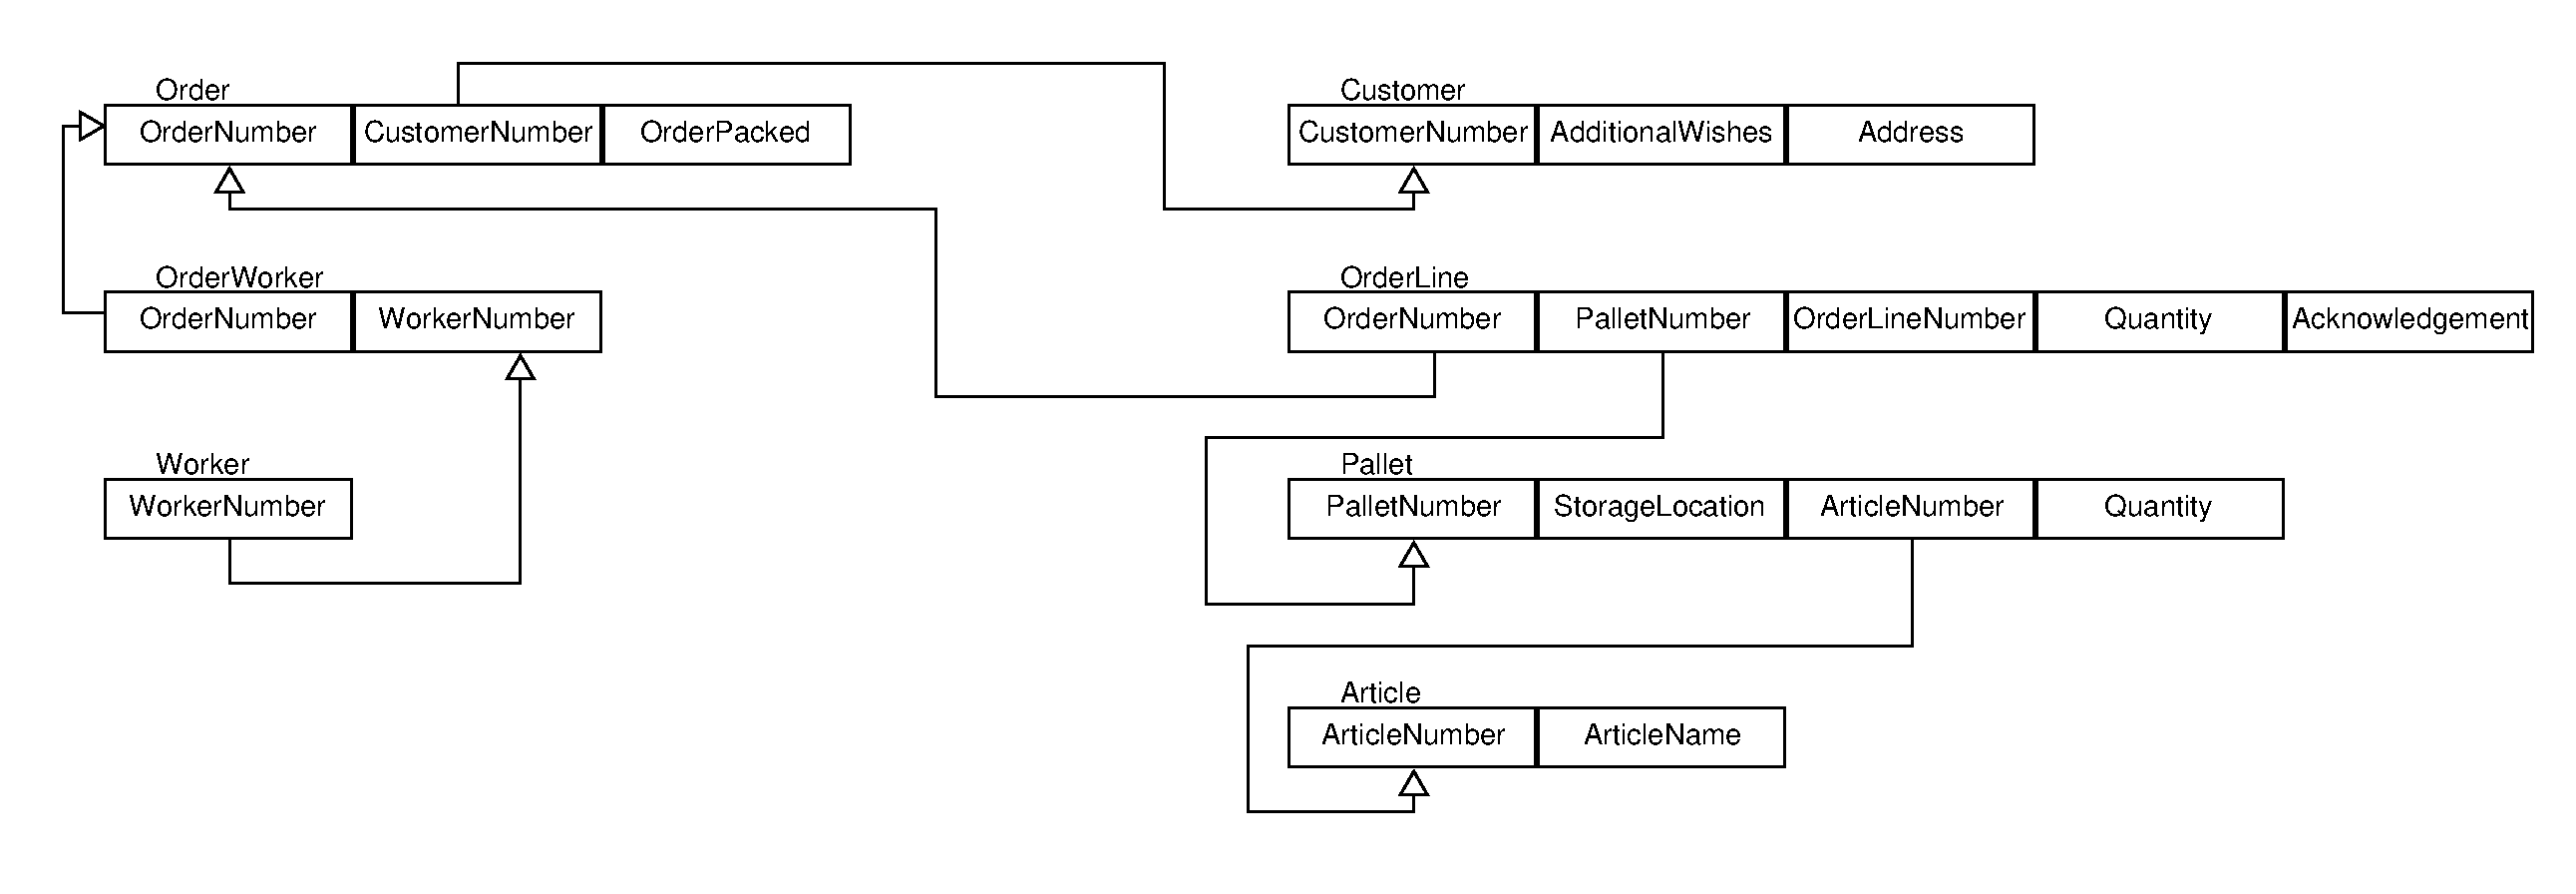
\includegraphics[width=\textwidth]{images/LogicalModel_MockWMS}
	\caption{Relational Schema Warehouse Database}
	\label{fig:LogicalModelWMS}
\end{figure}

For an actual warehouse the customers attributes would change completely, as companies might have multiple addresses, therefore that might change for every order of that customer, making it easier to add an address field to the order and not the customer.  Also a customer might want to add additional wishes just to a specific order or dependent on what might be ordered, therefore the additional wishes might also be moved to the order, but for a demo case, that is not executed at a pilot company, the model is sufficient.

\subsubsection{Interface}
The interface, that is exposed by the \gls{wms}, is a \gls{rest} interface, for the demo case this means that the communication layer, explained in subsection \ref{subsec:communication}, can be skipped, as the wearable chosen in section \ref{sec:processes} is able to connect to a \gls{rest} \gls{api} directly. And for a demo case the communication layer is also not needed to further transform or do similar things with the data that is passing through it. The options available through the \gls{rest} interface are the following:
\begin{description}
	\item[] \hfill \\
	\item[] \hfill \\
	\item[] \hfill \\
	\item[] \hfill \\
\end{description}


\textcolor{red}{Add information about database design, and rest api interfaces}


\subsection{Wearable | Application}
\textcolor{red}{Add information on how the wearable application works, maybe with web interface or direct implementation}

\textcolor{red}{add more sophisticated class diagram}

\section{Planning}
In the future for this task, there will be multiple wearables tried out and then decided which wearable will be used for the demo facility, as described in section \ref{sec:wearables}. Afterwards an application will be written for that wearable, to improve the process chosen in \ref{sec:processes}. 

This application will at least include the functionalities to:
\begin{itemize}
	\item Divide a given room in multiple sectors, to address a single part of the room with a given location string.
	\item Reset the case to allow multiple showcases of the demo.
	\item Allow scanning of \gls{id}s on \gls{parcel}s and pallets.
	\item Send confirmations to the \gls{wms}, that an action has been completed.
\end{itemize}

For the demo environment, an area will be rented that allows to place a rack in there with \gls{parcel}s. The \gls{parcel}s will be equipped with an \gls{id} that can be scanned with the chosen wearable.

When the implementation of the demo application is finished a second one could be started to show \gls{sme} the differences between the possibilities different wearables give the user.

\section{Conclusion}
\begin{frame}\frametitle{Conclusion}
	\begin{itemize}
		\item Reference Model
		\item Details Depend on Specific Cases
		\begin{itemize}
			\item Wearable
			\item Process
			\item Backend
		\end{itemize}
		\item 
	\end{itemize}
\end{frame}
\begin{frame}\frametitle{Reflection}
	\begin{itemize}
		\item Communication is problematic
		\item Small things can take more time than anticipated
	\end{itemize}
\end{frame}
\begin{frame}\frametitle{Future}
	\begin{itemize}
		\item Choosing Wearable
		\item Implementing Communication Layer
		\item Setting up Physical Environment
		\item Design and Develop Wearable Application
		\item Test Demo Case
	\end{itemize}
\end{frame}


\setbeamercolor{background canvas}{bg=matblue}
\setbeamercolor{normal text}{fg=white}
\begin{frame}[plain, b]
\centering
\huge \textcolor{white}{Thank You}
\normalsize

\vspace*{\fill}

 \begin{beamercolorbox}[wd=\paperwidth]{section in head/foot}
 \centering
Wearables in Logistics - Demo Facility
\vskip10pt
\end{beamercolorbox}
 \end{frame}

\end{document}
